\begin{quote}\small\textbf{观课提示}\quad 比较低频和高频模式，预测哪一项先衰减，再核对边界条件。

\href{https://www.youtube.com/watch?v=ToIXSwZ1pJU}{原课程视频}\quad\href{https://vitael04213.github.io/3blue1brown-notes/lessons/heat-equation.html}{本节网页与媒体}\quad\href{https://vitael04213.github.io/3blue1brown-notes/lab.html\#heat}{参数实验}
\end{quote}
\begin{figure}[htbp]\centering
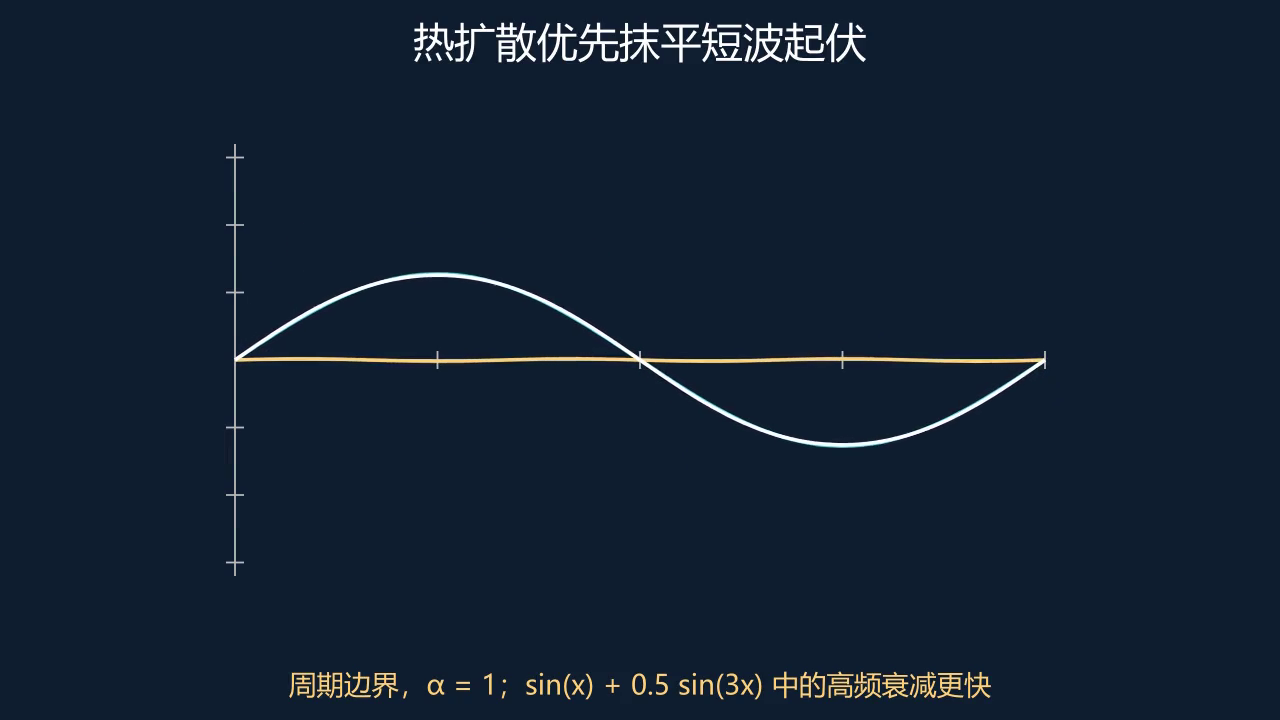
\includegraphics[width=0.98\linewidth]{figures/FourierHeat.png}
\caption{周期边界下，低频（蓝）与高频（黄）以不同速度衰减，白线为总和。本项目原创 Manim 动画关键帧；完整动画与操作入口见本节网页。}
\end{figure}
